\documentclass{article}
\usepackage{amsthm} 
\usepackage{physics}

\usepackage{ragged2e}
\usepackage{quoting}
\usepackage{pgfplots}
\pgfplotsset{compat=1.18}
\usetikzlibrary{decorations.pathmorphing}
\usepackage{circuitikz}
\usepackage{amsthm}
\usepackage{tabularx}
\usepackage[colorlinks=true, linkcolor=black]{hyperref}
\usetikzlibrary{shapes,decorations,shadows}
\usepackage[a4paper, left=1.5cm, right=1.5cm, top=2cm, bottom=2cm]{geometry}

\usetikzlibrary{shapes,arrows,positioning}
\title{Appunti laboratorio di elettromagnetismo}
\author{ Mirolo Manuele / Alessio Brusini}
\date{a.a. 2025/26}
\newtheorem{theorem}{Teorema}
\begin{document}
\maketitle
\justifying
\tableofcontents
\newpage
\section{Lezione 22/09/2025}
\subsection{Richiami di elettromagnetismo}
\begin{itemize}
    \item La carica elettrica è quantizzata, ovvero esiste una carica elementare $1 e = 1.6 \cdot 10^{-19} C$
    \item Legge di Coulomb, che descrive la forza repulsiva/attrattiva tra due cariche puntiformi:
    \[
    \vec{F}_{1,2} = \frac{Q_1 Q_2}{4\pi\epsilon_0 r^2}
    \]
    dove $\epsilon_0 = 8.85 \cdot 10^{-12} \frac{C^2}{N \cdot m^2}$ è la costante dielettrica del vuoto.
    
    Possiamo notare che il campo elettrico è conservativo, per cui esiste un \textit{potenziale elettrico} $V$: 

    \begin{equation*}
        V=\frac{Q}{4 \pi \epsilon_0 r} \quad \vec{F} = - \vec{\nabla} V 
    \end{equation*}

    \item Definiamo \textbf{corrente elettrica} attraverso una superfice delimitante 2 regioni di spazio, la cui unità di misura è l'Ampere (A), tramite:
    \[
    I = \frac{dQ}{dt}
    \]

    Vale la legge sperimentale detta \textit{1° legge di Ohm}:
    \[
    V = R I
    \]
    dove $R$ è la resistenza del conduttore, che dipende dalla sua natura e dalla sua geometria, da cui la \textit{2° legge di Ohm}:
    \[
    R= \int_{0}^{l} \frac{d\rho(l')}{\Sigma(l')} dl'
    \]
    dove $\rho$ è la resistività del materiale e $\Sigma$ è la sezione del conduttore.
    
    La sua unità di misura è l'Ohm ($\Omega$):
    \[
    1 \Omega = 1 \frac{V}{A}
    \]

    \item La resistività dipende dalla temperatura secondo la legge:
    \[
    \rho(T) = \rho_{20} [1 + \alpha (T - 20^\circ C)]
    \]

    \item Definiamo \textbf{potenza elettrica}, effettuando un lavoro L per spostare una carica fra due punti, come:
    \[
    W = \frac{dL}{dt} = V I = I^2 R = \frac{V^2}{R}
    \]

    \item In un atomo unico il potenziale atomico tende a 0 all'avvicinarsi del nucleo, mentre in un solido la funzione potenziale è periodica a causa della sovrapposizione dei potenziali atomici.
    \item Definiamo \textbf{circuito elettrico} un campo elettrostatico $\vec{F}$ conservativo, il lavoro lungo un percorso chiuso è nullo, introduciamo allora un potenziale U, con dU differenziale esatto.
    
    Se la forza elettrica è originata da una distribuzione di carica \textbf{Q}, definiamo il \textbf{campo elettrico} $\mathbf{\vec{E}(\vec{r})}$ in ogni punto dello spazio. Tale \textbf{Q} permette di spostare una carica di prova \textbf{q} in $\vec{r}$ con una forza $\vec{F_e}(\vec{r}) = q \vec{E}(\vec{r})$

    Si definisce una \textit{funzione differenza di potenziale} $\Delta U = q \Delta $ e $\vec{E}= -\vec{\nabla} V$

        \item In un sistema fisico isolato (es. \textit{maglia conduttrice}), la carica totale si conserva, ovvero $\Delta V_{tot} = 0$, da cui la \textbf{legge di Kirchhoff}:
    \end{itemize}
    
    \begin{theorem}
        La somma delle tensioni ai capi di una maglia è nulla.
    \end{theorem}
    \[
    \sum_{k=1}^{n} V_k = 0
    \]

\section{Lezione 25/09/2025}
A causa di Benjaming Franklin la corrente va dal polo positivo a quello negativo, in quanto si pensava che fossero cariche positive a spostarsi, non quelle \textbf{negative} come avviene nella realtà.
La corrente all'interno di un circuito rimane costante, per la legge della conservazione della carica.
 
Nel momento in cui la corrente incontra un \textit{nodo}, una biforcazione,
trova due vie possibile da percorrere, per la conservazione avremmo:
$I_{tot}= I_1 + I_2$ \\
\begin{center}
\begin{circuitikz}
    % Punto nodale principale
    \draw(0,0) node[circ] (A) {} 
        to[short, label=$I$] (2,0) node[circ, label=above:$N$] (B) {}
        to[short, label=$I_1$] (3,-1) node[circ] (C) {};
    
    % Collegamenti aggiuntivi
    \draw(B) to[short, label=$I_2$] (3,1) node[circ] {};
\end{circuitikz}
\end{center}
Finchè il circuito è un sistema isolato, le correnti prese con i loro segni seguono la seguente legge: 
\[
I_{tot} = \sum_{k=1}^{n} I_k \; \rightarrow \; \sum_{k=1}^{n} I_k-I_{tot}=\sum_{j=1}^{n+1} I_j =0
\]

Da cui la \textbf{2° legge di Kirchhoff}:  \\
\centering
\textit{se un circuito costituisce un sistema isolato, la somma
delle correnti entranti in un suo nodo è uguale alla somma delle correnti uscenti dallo stesso nodo}
\justifying


Queste leggi valgono in \textit{corrente continua}, ovvero quando la corrente non varia nel tempo. 

\begin{itemize}
    \item Definiamo la \textbf{forza elettromotrice} (f.e.m.) come la differenza di potenziale tra i due poli di un generatore, generata da fennomeni chimici quali le reazioni di ossido-riduzione.
In realtà non si tratta di una forza, ma il potenziale elettrico:
\[
V_{1i}= - k \frac{q_1 q_i}{r_{1i}} \rightarrow F_{1i} = - \nabla V_{1i} 
\]
Una d.d.p. può non essere in grado di mantenere una corrente costante, in quanto la resistenza del circuito può variare nel tempo (bastoncino caricato). Ma queste correnti non osccillanti lo possono diventare applicando lavoro.\\
\textbf{N.B} : non sempre un voltaggio di corrente è equivalente alla sua forza elettromotrice.  

\item La f.e.m. garantisce che la corrente scorra nel circuito, in quanto fornisce energia al sistema (che viene persa dagli elettroni che viaggiano nel cirucito e vengono deviati dagli urti). Per quest'ultimo motivo introduciamo la 
\textbf{resistenza} (R). Poichè l'elettrone fa "più fatica" se ci sono meno vie e possibile e se le "porte d'ingresso" sono più strette, si deve avere:
\[
R \propto \frac{l}{\Sigma}
\]
dove $\Sigma$ è l'area della sezione retta del conduttore.

Tramite prove sperimentali si introduce la \textbf{legge di Ohm} (nell'ipotesi di materiale omogeneo e di sezione costante):
\[
R= \rho \frac{l}{\Sigma}
\]
dove $\rho (\theta)$ è la resistività del materiale, che dipende molto da $T$; inoltre $L \propto T$ e $\Sigma \propto T^2$, ma tali effetti si compensano. Da cui:
\[
\rho(\theta) \simeq \rho_{\theta^*}(1 + \alpha (\theta - \theta^*))
\]
dove $\theta^*$ è la temperatura di riferimento, che cambia per ingegneri e fisici (solitamente in rete è $\theta=20^{\circ}$).

Da ciò deriva il fatto che $R \propto T$.

\item Per l'intensità invece avremo 
\[
I = \frac{V}{R} \rightarrow V = R I
\]
Tutte le leggi sono \textit{fenomenologiche}, non derivano da principi primi.
\end{itemize}
La formula più realistica che rappresenta la resistenza di un tratto di circuito è la seguente:
\[
R = \int_{l_1}^{l_2} \frac{\rho(l')}{\Sigma(l')} dl'
\]
ovvero un integrale curvilineo\\

\begin{center}
\begin{circuitikz}
    % Circuito base: pila + resistore
    \draw(0,0) to[battery1, l=$V$] (0,2)
          to[short] (2,2)
          to[R, l=$R_1$] (2,0)
          to[R, l=$R_2$] (0,0);
    
          \draw (2,0) node[circ, label=below:$B$] {};
            \draw (0,2) node[circ, label=above:$A$] {};
            \draw (0,0) node[circ, label=below:$C$] {};
\end{circuitikz}
\end{center}
Siccome supponiamo che il circuito sia un sistema isolato, valgono
\[
V_{tot} = V_{AB} + V_{BC} \quad I=VR_{eq} \rightarrow R_{eq} = R_1 + R_2
\]

\section{Lezione 29/09/2025}
\subsection{Resistenze in serie e parallelo}
Vediamo un altro tipo di circuito, che rappresenta un \textbf{partitore di correnti}
\begin{center}
\begin{circuitikz}
  \draw
  (0,0) to[battery1, l=$V$] (0,4)
  to[short] (2,4)
  to[R=$R_1$] (2,0)
  (2,4) to[short] (4,4)
  (4,4) to[R=$R_2$] (4,0)
  -- (0,0);
\end{circuitikz}
\end{center}


deve valore la legge di Kirchhoff (sistena isolato) e quella di Ohm:
\[
I=I_1+I_2 
\]
Poichè supponiamo che non ci siano altre resistenze (sistema ideale), la differenza di potenziale ai capi delle due resistenze deve essere la stessa (dalla legge di Ohm):
\[
\frac{V}{R_{eq}} = \frac{V}{R_1} + \frac{V}{R_2} \rightarrow \frac{1}{R_{eq}} = \frac{1}{R_1} + \frac{1}{R_2} = \frac{R_1 + R_2}{R_1R_2}
\]

Supponiamo di avere un solo alimentatore e dover far funzionare tre dispositivi, utilizziamo un \textbf{partitore di tensione}
\begin{center}
\begin{circuitikz}[american]

  \draw
    (0,0) node[left] {$A$} to[battery1,l=$V$] (0,-6) node[left] {$D$};
  \draw
    (0,0) -- (2,0)
      to[R=$R_1$, *-*] (2,-2) node[right] {$B$}
      to[R=$R_2$, *-*] (2,-4) node[right] {$C$}
      to[R=$R_3$, *-*] (2,-6) -- (0,-6);
\end{circuitikz}
\end{center}
ovvero un oggetto che permette di dividere la tensione in più parti, stabili nel tempo.


Chiamiamo \textit{corrente continua}, quella che rimane costante per un perio abbastanza lungo di tempo. 
\pagebreak
\subsection{Strumenti per misurare corrente e tensione}
Uno strumento per misurare delle variabili fisiche dovrebbe sempre dare una risposta \textit{lineare}.
Indichiamo con:
\begin{itemize}
\item $\vec{E}$ il campo elettrico,
\item $\vec{B}$ il campo magnetico,
\item $\vec{F_L}$ la forza di Lorentz:
\end{itemize} 
\[
\vec{F_L} = q \vec{E} + q \vec{v} \times \vec{B}
\]
La forza di Lorentz subita da una carica in un campo elettromagnetico è la somma della forza elettrica e della forza magnetica, l'una moltiplicata per la carica e l'altra per la velocità della carica.

Sono tutte quantità relativisticamente invarianti dunque la formula vale sia per la fisica classica che per quella relativistica.

Consideriamo ora il caso di una calamita con i poli avvicinati e presente uno spazio cilindrico tra di loro. Se inseriamo li un segmento cilindrico di ferro dolce (materiale che reagisce velocemente al campo magnetico in cui si trova), allora posso trovare dei segmentini di linee di campo (che ricordiamo essere
ortogonali alla superfice equipotenziale della calamita) 

\begin{center}
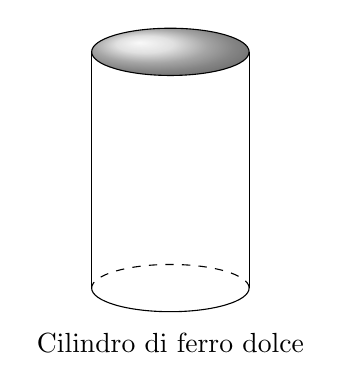
\begin{tikzpicture}
    
% Cilindro (vista 3D semplificata)
\shade[ball color=gray!40, opacity=0.8] (0,0) ellipse (1 and 0.3); % parte superiore
\draw (0,0) ellipse (1 and 0.3); % bordo superiore

\draw (-1,0) -- (-1,-3); % lato sinistro
\draw (1,0) -- (1,-3);   % lato destro

\draw (-1,-3) arc[start angle=180, end angle=360, x radius=1, y radius=0.3]; % base visibile
\draw[dashed] (1,-3) arc[start angle=0, end angle=180, x radius=1, y radius=0.3]; % base nascosta

% Etichetta
\node at (0,-3.7) {Cilindro di ferro dolce};

\end{tikzpicture}
\end{center}

Se supponiamo di avvolgere tale cilindro con una spira e facciamo passare corrente elettrica, chiamati a e b i lati corto e lungo della spira e 
osservando il più classico degli \textit{elettroni di conduzione} con velocità $v$, il tratto di spira a sarà ortogonale al campo magnetico 
\[
e^- v \times B = e^- v B 
\]
L'elettrone viene "spinto fuori dalla spira"

Contrariamente nel tratto b, l'elettrone non viene deviato, in quanto la velocità è parallela a $B$. Tornato nel tratto A, se I rimane costante avremo nuovamente $\vec{F_L}$, sempre diretta verso l'esterno.

Questa coppia di forze genera un \textit{momento torcente} pari a: $\tau = e^- v B b $

Il flusso invece è dato dalla \textit{densità dei portatori di carica} $\lambda$, dunque scrivendo la corrente come $ v \lambda e =I = \frac{dq}{dt}$, da cui
\[
\tau = n B I a b
\]
dove $n$ è il numero di spire attorno al magnete. 
Bilanciamo questo momento con una forza elastica grazie a delle molle elicoidali controrotanti (in modo da bilanciare le imperfezioni), ricordando che (nell'approsimazione di $\theta < 4^\circ$):
\[
\tau_{el} \approx k \theta = \tau_{mag} = B I b \rightarrow \theta = \frac{B n a b}{k} I
\]
Dobbiamo dunque risaltare il nostro segnale, per questo la molla ha più spire (non più di 10 per evitare deformazioni), in tal modo inoltre, l'approsimazione angolare vale fino a $\theta < 40^\circ$ (max $\theta = 3600^\circ$).

Nel caso della realtà abbiamo il cosidetto \textit{effetto Joule}, ovvero il riscaldamento del conduttore, quindi posso usare solo piccole correnti 
Lo strumento appena descritto è detto \textbf{Amperometro}, costruendo un circuito con una resistenza e un amperometro in parallelo, possiamo misurare la corrente che passa nel circuito.
avremmo
\[
I= I_A + I_S= \frac{V}{R_A}+ \frac{V}{R_S}
\]
costruiamo la resistenza in modo che $R_A << R_S$ (per esempio $\frac{R_A}{R_S}=\frac{1}{10}$), tali $R_S$ sono dette \textbf{resistenze di shunt}. La precisione, dunque, diminuisce in modo direttamente proporzianale all'aumento del numero di resistenze 

\section{Lezione 02/10/2025}
Chiediamoci quale sia la $\Delta V$ ai capi di una resistenza e consideriamo la resistenza Ohmica $V_{AB}= IR$

\begin{center}
\begin{circuitikz}
  \draw
  (0,0) to[battery1, l=$V$] (0,4)
  to[short] (2,4)
  to[R=$R_1$] (2,0)
  (2,4) to[short] (4,4)
  to[R=$R_2$] (4,2) 
  to[rmeter, t=A] (4,0)
  -- (0,0);
\end{circuitikz}
\end{center}
Per farlo utilizziamo un amperometro, ma in tal modo lo perturbiamo, avremo $R<R^*$, per rendere la situazione accettabile aggiungiamo una resisteza prima dell'amperometro, tale che
$R_2>>R$, potendo trascurare la corrente che passa nell'amperometro.

Dunque misuro la d.d.p.\ teorica rispetto a quella reale (con lo strumento di misura):
\[
V_{AB}=IR \quad V^*_{AB} = I \frac{R R_A}{R + R_A} 
\]
\[
\frac{V_{AB}- V^*_{AB}}{V_{AB}}= \text{errore dovuto all'amperometro}
\]
Ponendo $R_A$ come somma di $R_2$ e quella dovuta all'amperometro.

Posso anche utilizzare un voltimetro, che lavora fra due materiali conduttori di resistenza trascurabile; uno strumento è il voltimetro a fogli conduttori, che in base all'angolo di inclinazione delle mie mie piastre mi indichi la $\Delta V$.

\subsection{Come misurare una resistenza}
Nell'ipotesi che tale resistenza sia ohmica, dunque $R=\frac{V}{I}$ (caso ideale, non reale), ottenendo così una scala iperbolica (essendo $V$ costane e $I$ variabile). 
A causa della degradazione della batteria dello strumento erogatore della forza elettromotrice, ottengo un errore di sottostima su $R$.

Un altro modo per misurare la resistenza è utilizzare un generatore regolabile, mettere in parallelo la resistenza con un voltimetro e in serie ai due un amperometro.
\begin{center}
\begin{circuitikz}[american]
    % Generatore di tensione variabile
    \draw (0,0) to[battery1] (0,2);
    \draw (0,2) -- (2,2);
    % Amperometro
    
    
    % Resistenza
    \draw (2,2) to[R, l=$R$, v=$V_R$] (2,0);
    
    % Collegamento di ritorno
    \draw (2,0) -- (0,0);
    
    % Voltmetro in parallelo alla resistenza
    \draw (2,2) to[rmeter, t=V] (4,2);
    \draw (4,2) -- (4,0);
    \draw (4,0) -- (2,0);
    
    \draw (0,0) to[rmeter, t=A] (2,0);

\end{circuitikz}
\end{center}
Posso disegnare un grafico \textit{V su I}, successivamente cerco di ricavare la legge fisica, ciò che mi aspetto è un andamento lineare, dove $\frac{1}{m}=R$
Inoltre, a causa dell'effeto Joule si comincia a perdere la linearità, sostituita da un andamento logaritmico

\subsection{La qualità di una pila}
La bontà di una pila è data dal fatto che anch' essa ha una resistenza interna, tanto più è bassa, migliore è la pila.
Quando la pila inizia a consumarsi, la resistenza interna della pila aumenta a causa di fenomeni di ossidazione o sbalzi termici. 

Per misurare lo stato della pila creo un circuito con essa e:
\begin{itemize}
\item un amperometro in serie alla pila (prima)
\item una resistenza incognita, devo creare la più grande resistenza con quelle a disposizione (le metto in serie) ($R_x = \sum_{i=1}^{n} R_i$)
\item un voltimetro in parallelo alla pila
\end{itemize} 
\begin{center}
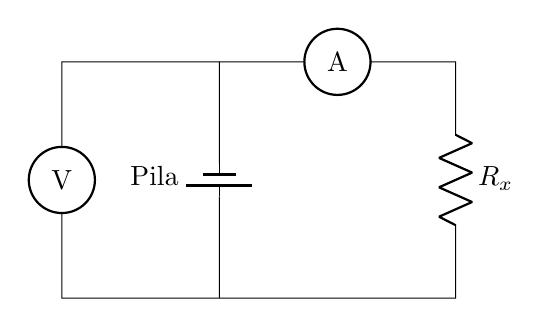
\begin{tikzpicture}
  \draw
  (0,0) to[battery1, l=Pila, name=pila] (0,3)
        to[rmeter, t=A] (3,3)
        to[R, l=$R_x$] (3,0)
        to[short] (0,0);
  
  % Voltmetro in parallelo alla pila
  \draw (0,3) to[short] (-2,3)
        to[rmeter, t=V] (-2,0)
        to[short] (0,0);
\end{tikzpicture}
\end{center}
Creo un grafico $V$ su $I$, aumentando la resistenza, ottengo un andamento iperbolico sul primo quadrante (grazie al cazzo). 
Nel momento in cui incontro un andamente lineare ("inversamete lineare") ho un comportamento ohmico, che facendo il fit lineare (sul sottoinsieme di dati ideale) posso ottenere il valore della resistenza interna della pila. 

Estrapolando a $I=0$ ottengo il valore della $\Delta V$ della pila. Con una pila nuova dovrei ottenere una linea orizzontale ad un certo valore di $V$.

\section{Lezione 09/10/2025}
\subsection{Misura della resistenza}
Una tecnica molto utilizzata è la \textit{misura di zero}, che sono le più precise che si possono fare, in questo caso chiameremno 
\textbf{misura a ponte di Wheatstone}
\begin{center}
\begin{circuitikz}
\draw
(0,0) to[battery1, l=$V$] (0,4)
to[short] (2,4)
to[R=$R_1$] (2,2)
to[R=$R_2$] (2,0)
to[short] (0,0)

(2,4) to[short] (4,4)
to[R=$R^*$] (4,2)
to[R=$R_3$] (4,0)
to[short] (2,0)

(2,2) to[rmeter, t=A] (4,2);

\node[above] at (2,4) {$A$};
\node[left] at (2,2) {$B$};
\node[right] at (4,2) {$C$ };
\node[below] at (2,0) {$D$};
\end{circuitikz}
\end{center}
Le resistenze erano ottenute mettendo nelle loro posizioni dei \textit{reostati}, per ottenere $R^*$ si ottiene "giocando" con le resistenze fino ad azzerrare l'amperometro,
infatti:
\begin{itemize}
  \item se fra B e C non passa corrente vuol dire $\Delta V_{BC}=0$
  \item quindi fra A-B e A-C avremo la stessa $\Delta V$, $ \Delta V_{AB}= \Delta V_{AC}$, ma avremmo anche $\Delta V_{BD} = \Delta V_{CD}$ (Kirchhoff)
  \item se la $R^*$ obbedisce alla legge di Ohm (trascurando l'effetto Joule), avremmo
  \[
  \Delta V_{AB}=IR \quad\Delta V_{AC}=I^*R^* \quad \Delta V_{BD}=I_2R_2 \quad \Delta V_{CD}=I_3R_3
  \]
  ottenendo un sistema 
  \begin{equation}
    \begin{cases}
      I_1R_1=I^*R^*\\
      I_2R_2=I_3R_3\\
    \end{cases}
  \end{equation}
  \item se considdero la corrente $I_A = 0$ allora avrò che le correnti sul stesso ramo della maglia sono uguali ($I_1=I_2 \quad I_*=I_3$).
  \item facendo il rapporto membro a membro di (1) ottengo: \[R^*=R^3 \frac{R_1}{R_2}\]
\end{itemize}
\pagebreak
\subsection{Condensatori}
Lo assumiamo come un accomulatore di cariche elettriche che inserieamo nel circuito.

Supponiamo di avere un \textbf{segnale elettrico} ovvero una variazione di $\Delta V$ nel tempo $t$, se
\begin{enumerate}
  \item la carica associata al segnale viene portata al condensatore (grazie ad uno \textit{spinotto}), esso si carica in modo logaritmico;
  \item  si ferma il caricamento;
  \item  si fa partire un altro cirucito, che fa scaricare il più linearmente possibile il condensatore (l'amdamento sarà esonenziale decrsecnte approssimabile al prim'ordine a una retta).
  \item se carico il condensatore con un diverso segnale allora avrò una retta con la stessa pendenza ma che incontra lo zero della carica del condensatore in un punto diverso.
  \item iterando il procedimento posso contare il numero di volte in cui un \textit{clock} ha segnato lo scaricamento parziale del condensatore
  
  Il numero di segnali è direttamente proporzionale al $t$ necessario per scaricare il condensatore
  \item se inoltre il $t$ di scarica è associato al segnale (a sua volta associata al tempo di carica), allora posso creare una relazione tra la carica e il tempo di carica ($\frac{C}{s}=A$)
\end{enumerate}
Su questo procedimento si basa il funzionamento dell'amperometro

\subsection{$1^\circ$ Esperienza di laboratorio}
Utilizzeremo un circuito composto da 
\begin{itemize}
  \item una resistenza
  \item una lampadina a filamento, composta da:
   \begin{itemize} 
    \item un bulbo di vetro (da cui si può aspirare aria per sostituirla con qualche milli Bar di un gas nobile) 
    \item due filamenti collegati al circuito e ad un altro filamentino (acciaio tungstenato), tramite l'effetto Joule viene prodotta illuminazione
   \end{itemize}
   \item in parallelo alla lampadina un voltmetro
  \item un amperometro
\end{itemize}
\begin{center}
\begin{circuitikz}[american]
    % Generatore di corrente continua variabile a sinistra
    \draw (0,0) to[battery1] (0,3);
    
    % Resistenza in alto
    \draw (0,3) to[R, l=$R$] (3,3);
    
    % Lampadina a destra
    \draw (3,3) to[lamp, l=$L$] (3,0);
    
    % Amperometro in basso
    \draw (0,0) to[rmeter, t=A] (3,0);
    
    \draw (3,2) to[short] (4.5,2) 
    % Voltmetro in parallelo alla lampadina
    to[rmeter, t=V] (4.5,1)
    to[short] (3,1);
\end{circuitikz}
\end{center}
L'obbiettivo è quello di costruire una curva voltamperrometrica ($I$ vs $V$), se la lampadina rispetta la legge di Ohm allora mi aspetto un andamento lineare.

L'andamento reale è più esponenziale  (sotto la linea retta ideale) ($I \propto V^2$), questo accade perchè il sistema fisico non è isolato (non tutta la f.e.m. crea corrente), 
infatti nel metallo della lampadina si crea attrito (emissione nell'infrarosso), l'elettrone di conduzione si muove in modo erratico (a causa degli scontri con gli elettroni degli atomi del metallo).
Si formano, incoerentemente, dei fotoni i quali creano delle differenze nel campo elettrico. Difatti, gli elttroni dell'atomo possono eccitarsi e cambiare orbitale. L'atomo eccitato ritorna allo stato fondamentale
dopo circa $10^{-8}s$, l'energia liberata forma i fotoni con frequenze nel visibile:
\[ E_{\gamma}= h \nu \]

Se uno degli $e^-$ di conduzione riesce ad eccitare gli elettroni di un atomo della mia resistenza interna alla lampadina, allora dopo riesco a produrre una luminescenza (transiente, tranzione di fase). 
Abbiamo individuato un \textit{fenomeno a soglia} (che si verifica solo quando un determinato parametro supera un valore critico preciso, in questo caso l'energia)

Supponiamo che a $V^*$ inizia tale fenomeno, da qui in poi la conduzione nel circuito cambia (inizia il comportamento logaritmico), infatti l'energia che io fornisco sotto forma di f.e.m. verrà assorbita e poi dissipata. 

La differenza fra la curva e la retta ideale continua ad aumentare fino al bruciare del filamento (il metallo bolle), ovvero un po' di metallo diventa gas dentro se stesso, 
il filamento si gonfia (aumenta la resistenza, sia perchè è più caldo, sia perchè è diminutia l'area della sezione retta in alcuni punti).

Al bruciare del filamento $I=0$, ma la zona subito prima precedenta da questa decaduta è di transione di fase (scioglimento e rottura). In realtà anche nella prima transizione di fase (inizio emissione fotoni), ci sono delle 
piccole oscillazioni che però non sono visibili. 

\textbf{N.B.}: durante le transioni di fase ci sono delle fluttuazioni negli osservabili, nel nostro caso ciò è dovuto allo scambio energetico, che modifica la resistenza (osservabile) del filamento.
In generale i fenomeni di transizione sono associati oscillazioni nelle osservabili. 
Sapendo che $R=\frac{1}{m}=\frac{\Delta V}{\Delta I}$, questi $\Delta$ sono dati dalle spezzate che collegano i nostri punti.
Questa resistenza, detta \textit{resistenza dinamica}, fluttua molto nel momento delle tranzioni di fase 





\begin{center}
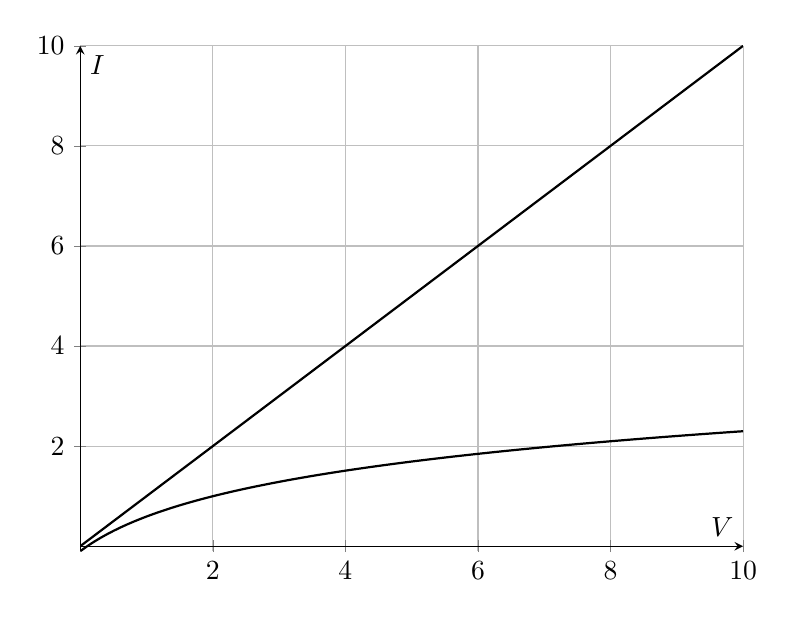
\begin{tikzpicture}
\begin{axis}[
    axis lines = middle,
    xlabel = $V$,
    ylabel = {$I$},
    xmin = 0,
    xmax = 10,
    ymin = -0.1,
    ymax = 10,
    grid=both,
    width=10cm,
    height=8cm,
    legend pos=north west
]
\addplot [
    domain=0:10,
    samples=100,
    color=black,
    thick
] {x};
\addplot [
    domain=0:10,
    samples=100,
    color=black,
    thick
] {ln(x+1)-0.1};
\end{axis}
\end{tikzpicture}
\end{center}

\begin{center}
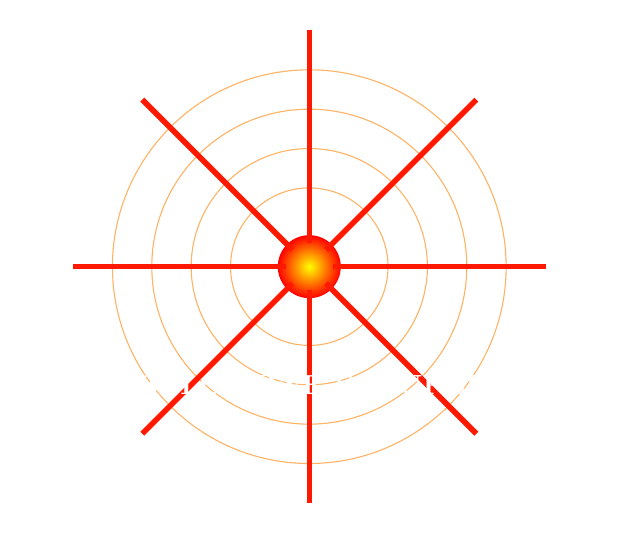
\begin{tikzpicture}
% Nucleo
\shade[inner color=yellow, outer color=red] (0,0) circle (0.4cm);

% Esplosione
\foreach \r in {1,1.5,2,2.5}
  \draw[orange, opacity=0.6] (0,0) circle (\r cm);

% Raggi principali
\foreach \a in {0,45,90,135,180,225,270,315}
  \draw[red!80!orange, line width=2pt] 
    (\a:0.3) -- (\a:3);

\node[white] at (0,-1.5) {black! \textbf{ESPLOSIONE DI SUPERNOVA}};
\end{tikzpicture}
\label{fig:esplosione}[esplosione di supernova]
\end{center}

La polarizzazzione risulta ininfluente per il nostro sistema fisico 


\pagebreak
\section{Lezione 13/10/2025}
\subsection{Come fare la relazione}
\begin{itemize}
  \item titolo
  \item preambolo: breve descrizione dell'esperienza
  \item tabelle (brevi, 7 righe e 4 colonne e in allegato se molto lunghe)
  \item descrizione dell'apparato sperimentale se i dati dipendono fortemente dall'apparato
  \item grafici (che mostrano l'andamento fisico);\\ stessa dimensione del carattere della relazione sugli assi; \\barre d'errore per ogni punto (se pochi punti), altrimento si inseriscono ogni 3/4 punti. 
  \item commenti sui grafici (più quantitativi possibile)
  \item osservazioni sui risultati attesi e confronto con quelli ottenuti (citare le fonti d'errore)
  \item se i risultati sono in linea con le aspettative si può commentare questo fatto, aggiungendo dati numerici che verificano quest'ipotesi
\end{itemize}
\subsection{Semiconduttori}
La disposizione degli elettroni negli atomi di un conduttore presenta abbassamenti di potenziale all'avvicinarsi al nucleo dell'atomo contiguo. Dunque, la maggior parte degli elettroni si trova  
al di sopra di una certa soglia di energia. Alcuni elettroni si trovano 2/3 $eV$ al di là di questa soglia,  andando ad eccitare questi nuclei (es. scaldando gli elettroni) il materiale può diventare un conduttore, superando le buche di potenziale, 
questi materiali sono detti \textit{semiconduttori}. Essendo la barriera energetica di pochi $eV$, allora una bassa differenza di temperatura produce una grande quantità di elettroni disponibili per la conduzione elettrica. 

Alcuni materiali di questo tipo sono il silicio (Si) e il Germanio (Ge). Essi sono atomi \textit{tetravalenti}, dunque formano strutture nei cristalli tetraedici (ognuno è legato con altri 4 atomi). 

All'interno di questi materiali si possono già trovare degli elettroni liberi, circa $\frac{1e}{10^6 \text{atomi}}$, che aiutano la conduzione. 

Quanto un elettrone di conduzione si slega dalla sua nicchia, allora oltre alla carica negativa si crea anche una \textit{lacuna}, che è l'equivalente di una carica positiva che ha modulo opposto a quello dellla carica negativa.
la lacuna viene occupata da un elettrone vicino, che a sua volta lascia una lacuna, creando una corrente.

Si individuano così 2 tipi di conduzione:
\begin{itemize}
  \item conduzione per elettroni liberi (fluttuazioni termiche)
  \item conduzione per lacune (passaggio in \textit{banda di conduzione})
\end{itemize}
La differenza energetica fra i campi elettrici dei materiali è peculiare per ognuno di essi, avvicinando i due si creano della possibilità di "travaso" degli elettroni.
Si usa, per favorire ciò, il \textbf{drogaggio}, ovvero l'inserimento di atomi di un altro materiale con un diverso numero di valenza (tri/pentavalenti), così da creare una lacuna o un elettrone libero. 
\begin{itemize}
    \item L'assorbimento di questi materiali avviene per \textit{diffusione}, creando un surplus di elettroni liberi o lacune
    \item  Prima dell'inizio della diffusione i materiali sono intrisicamente neutri, solo successivamente si accumulano cariche
    \item  La regione di contatto fra i materiali è detta \textbf{giunzione}
    \item  La condizione d'equilibrio si raggiunge quando la quantità di cariche si stabilizza (ma lo scambio continua sempre ad esserci)
    \item Lo spazio sulla giunzione è detto \textbf{zona di svuotamento}, in cui non ci sono più cariche libere di muoversi (al meno di motivi termici), di cui valuteremo lo spessore.
    \item L'oggetto che si ottiene con questo processo si chiama \textbf{diodo}
\end{itemize}

Tutto ciò avviene in una decina di secondi.


\begin{center}
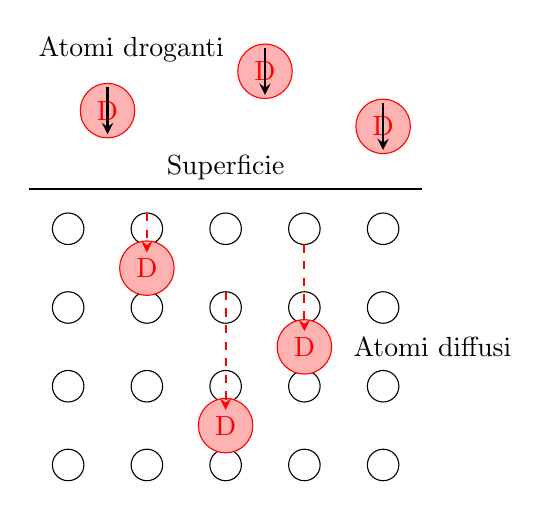
\begin{tikzpicture}[
    atom/.style={circle, draw, minimum size=0.4cm},
    dopant/.style={circle, draw, red, fill=red!30, minimum size=0.4cm},
    surface/.style={thick},
    arrow/.style={->, >=stealth, thick}
]

% Materiale di base (es. silicio)
\foreach \x in {0,1,2,3,4} {
    \foreach \y in {0,1,2,3} {
        \node[atom] at (\x, \y) {};
    }
}

% Superficie
\draw[surface] (-0.5, 3.5) -- (4.5, 3.5);
\node[above] at (2, 3.5) {Superficie};

% Atom drogante che si avvicina
\node[dopant] (d1) at (0.5, 4.5) {D};
\node[dopant] (d2) at (2.5, 5) {D};
\node[dopant] (d3) at (4, 4.3) {D};

% Frecce che indicano il movimento
\draw[arrow] (0.5, 4.8) -- (0.5, 4.2);
\draw[arrow] (2.5, 5.3) -- (2.5, 4.7);
\draw[arrow] (4, 4.6) -- (4, 4);

% Atom drogante già diffusi
\node[dopant] at (1, 2.5) {D};
\node[dopant] at (3, 1.5) {D};
\node[dopant] at (2, 0.5) {D};

% Frecce di diffusione interna
\draw[arrow, red, dashed] (1, 3.2) -- (1, 2.7);
\draw[arrow, red, dashed] (3, 2.8) -- (3, 1.7);
\draw[arrow, red, dashed] (2, 2.2) -- (2, 0.7);

% Etichette
\node[above right] at (-0.5, 5.0) {Atomi droganti};
\node[right] at (3.5, 1.5) {Atomi diffusi};


\end{tikzpicture}
\end{center}

Inserendo il diodo in un circuito possiamo creare 
\begin{itemize}
\item una \textbf{polarizzazione inversa} con generatore la cui corrente passa in discordia alla carica nel diodo, tale processo:
\begin{itemize}
    \item  aumenta la quantità di cariche da una parte e dall'altra
    \item diminuisce la zona di svuotamento
    \item vi è minor passaggio di corrente, e quella che passa lo fa a causa di movimenti termici
\end{itemize}
\item una \textbf{polarizzazione diretta} se la corrente del generatore va nella stessa direzione della carica nel diodo, in questo caso la zona di svuotamento aumenta
\end{itemize} 

\begin{minipage}{0.45\textwidth}
\begin{center}
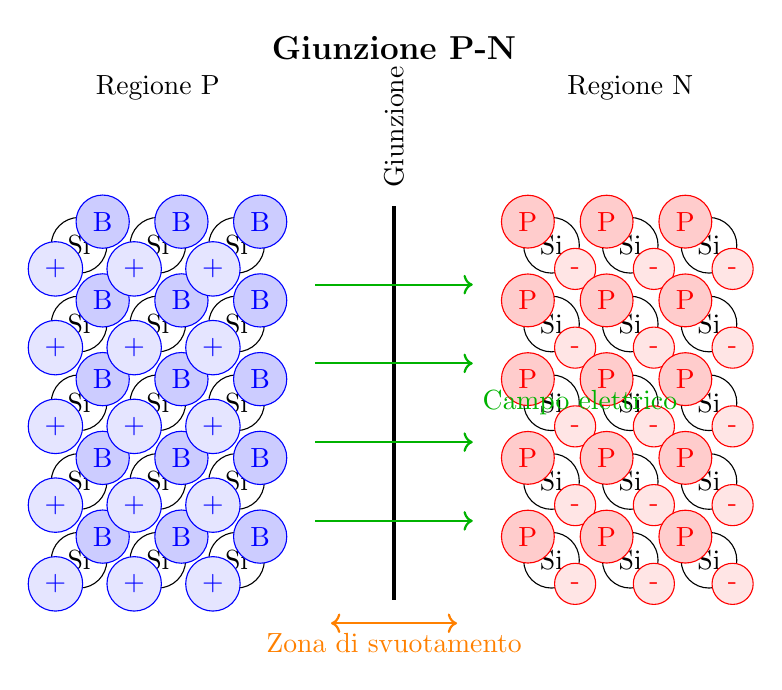
\begin{tikzpicture}[
    atom/.style={circle, draw, minimum size=0.5cm},
    acceptor/.style={circle, draw, blue, fill=blue!20, minimum size=0.5cm},
    donor/.style={circle, draw, red, fill=red!20, minimum size=0.5cm},
    electron/.style={circle, draw, red, fill=red!10, minimum size=0.3cm},
    hole/.style={circle, draw, blue, fill=blue!10, minimum size=0.3cm},
    charge/.style={rectangle, draw, minimum width=0.3cm, minimum height=0.1cm}
]

% TITOLO
\node[align=center, font=\large\bfseries] at (0, 6.5) {Giunzione P-N};

% REGIONE P (sinistra)
\node[align=center] at (-3, 6) {Regione P};
\foreach \x in {-4,-3,-2} {
    \foreach \y in {0,1,2,3,4} {
        \node[atom] at (\x, \y) {Si};
        \node[acceptor] at (\x+0.3, \y+0.3) {B};
        \node[hole] at (\x-0.3, \y-0.3) {+};
    }
}

% REGIONE N (destra)
\node[align=center] at (3, 6) {Regione N};
\foreach \x in {2,3,4} {
    \foreach \y in {0,1,2,3,4} {
        \node[atom] at (\x, \y) {Si};
        \node[donor] at (\x-0.3, \y+0.3) {P};
        \node[electron] at (\x+0.3, \y-0.3) {-};
    }
}

% GIUNZIONE
\draw[ultra thick] (0, -0.5) -- (0, 4.5);
\node[rotate=90] at (0, 5.5) {Giunzione};

% CAMPO ELETTRICO
\foreach \y in {0.5,1.5,2.5,3.5} {
    \draw[->, thick, green!70!black] (-1, \y) -- (1, \y);
}
\node[green!70!black, right] at (1, 2) {Campo elettrico};

% ZONA DI SVUOTAMENTO
\draw[<->, thick, orange] (-0.8, -0.8) -- (0.8, -0.8);
\node[orange, below] at (0, -0.8) {Zona di svuotamento};

\end{tikzpicture}
\end{center}
\end{minipage}
\hfill
\begin{minipage}{0.45\textwidth}
\begin{center}
\begin{circuitikz}[american]
    \node[align=center, font=\large\bfseries] at (3, 4) {Polarizzazzione inversa};
    % Batteria
    \draw (0,0) to[battery1, l=$V$] (0,2);

    % Collegamenti verso il rettangolo
    \draw (0,2) -- (0,3.5);
    \draw (0,3.5) -- (3,3.5);
    \draw (3,3.5) -- (3,3.0);
    \draw (0,0) -- (0,-1.5);
    \draw (0,-1.5) -- (3,-1.5);
    \draw (3,-1.5) -- (3,-1.0);


    \begin{scope}[shift={(4,-3)}, rotate=90]
    % Rettangolo (conduttore)
    \draw[thick] (2,0) rectangle (6,2);

    % Cariche positive a sinistra
    \foreach \y in {0.4, 1, 1.6} {
        \node at (2.4,\y) {\large $+$};
        \node at (2.8,\y) {\large $+$};
    }

    % Cariche negative a destra
    \foreach \y in {0.4, 1, 1.6} {
        \node at (5.2,\y) {\large $-$};
        \node at (5.6,\y) {\large $-$};
    }

    % Frecce del campo elettrico
    \foreach \y in {0.4, 1, 1.6} {
        \draw[->, blue, thick] (3.2,\y) -- (4.8,\y);
    }
    \end{scope}
\end{circuitikz}
\end{center}
\begin{center}
\begin{circuitikz}[american]
    \node[align=center, font=\large\bfseries] at (3, 4) {Polarizzazzione diretta};
    % Batteria
    \draw (0,0) to[battery1, invert, l=$V$] (0,2);

    % Collegamenti verso il rettangolo
    \draw (0,2) -- (0,3.5);
    \draw (0,3.5) -- (3,3.5);
    \draw (3,3.5) -- (3,3.0);
    \draw (0,0) -- (0,-1.5);
    \draw (0,-1.5) -- (3,-1.5);
    \draw (3,-1.5) -- (3,-1.0);


    \begin{scope}[shift={(4,-3)}, rotate=90]
    % Rettangolo (conduttore)
    \draw[thick] (2,0) rectangle (6,2);

    % Cariche positive a sinistra
    \foreach \y in {0.4, 1, 1.6} {
        \node at (2.4,\y) {\large $-$};
        \node at (2.8,\y) {\large $-$};
    }

    % Cariche negative a destra
    \foreach \y in {0.4, 1, 1.6} {
        \node at (5.2,\y) {\large $+$};
        \node at (5.6,\y) {\large $+$};
    }

    % Frecce del campo elettrico
    \foreach \y in {0.4, 1, 1.6} {
        \draw[<-, blue, thick] (3.2,\y) -- (4.8,\y);
    }
    \end{scope}
\end{circuitikz}
\end{center}
\end{minipage}


\pagebreak
Creando un circuito di questo tipo
\begin{center}
\begin{circuitikz}[american]
    
    % Generatore di corrente continua variabile a sinistra
    \draw (0,0) to[battery1, invert, l=$V$] (0,3);
    
    % Resistenza in alto
    \draw (0,3) to[R, l=$R$] (3,3);
    
    % Lampadina a destra
    \draw (3,3) to[diode, ] (3,0);
    
    % Amperometro in basso
    \draw (0,0) to[rmeter, t=A] (3,0);
    
    \draw (3,2) to[short] (4.5,2) 
    % Voltmetro in parallelo alla lampadina
    to[rmeter, t=V] (4.5,1)
    to[short] (3,1);
\end{circuitikz}
\end{center}
mi aspetto che la corrente tenda ansotiticamente ad un certo $I_0$ per correnti negative, per correnti positive invece la corrente cresce esponenzialmente (le curve sono tipiche per un certo valore di temperatura).
La formula che mi descrive questo andamento è (per un diodo idelae)
\[
\displaystyle I(V)= I_0 e^{(\frac{qV}{\eta kT})} - 1
\]
dove $\eta$ è un parametro adimensionale che dipende dal materiale.

Al crescere della temperatura la curva "aumenta la sua pendenza", mentre $I_0$ diminuisce (più grande in modulo). Ho l'andamento opposto se diminuisco la temperatura, in tal caso, infatti, la resistenza interna 
del diodo aumenta. 

\begin{itemize}
\item $I_0$ dipende dalla temperatura:
\[
\displaystyle I_0 \propto KT^\alpha e^{-\frac{qV_G}{kT}}
\]
con $\alpha \in (1,2]$ e $K$ costante
i due segni all'argomento dell'espnenziale si "cancellano"


\item Anche se stiamo applicando una polarizzazione inversa (tensione negativa), poiché il comportamento è Ohmico, la curva caratteristica sarà completa e simmetrica. Potremo quindi ricostruire l'intero comportamento, inclusa la parte di polarizzazione diretta, semplicemente per simmetria.
\item Mettendo il diodo in un bagno per mantenere la temperatura costante, posso rilevare sul grafico i punti di intersezione fra certi valori $I^*$ e $V^*$. Con questi valori posso fare un altro grafico 
$V$ vs $T$, da cui osservo che, al decrescere della temperatura la tensione aumenta, ed è ciò che si osserva in un diodo reale, tale oggetto dunque riesce a mettere in correlazione lineare
la $T$ con una variabile da me controllabile ($V$). Quindi è sufficente un sistema, che, fissata una corrente, mi fornisca la tensione del circuito per sapere la temperatura del diodo.

\item Prendendo 3 valori di corrente, se il diodo è ideale, mi aspetto che aumentando $I$  $V$ aumenti linearmente, questo vale finchè non raggiungo temperature tali da cambiare la natura del materiale del diodo
\end{itemize}
\subsection{Come fare il fit esponenziale}
Poichè sappiamo fare un fit lineare possiamo linearizzare la nostra equazione, prendendo valori di $V$ tale che l'argomento dell'esponente sia maggiore di 1 posso usare
 \[
 I(V) \simeq I_0 e^{(\frac{qV}{\eta kT})} \rightarrow \log(I) = \log(I_0) + \frac{qV}{\eta kT}
 \]
 dunque sto facendo un fit in scala semilogaritmica da cui
 \begin{itemize}
  \item ottengo il valore di $\log(I_0)$ 
  \item conoscendo $q$ $ k$ e $T$ posso ottenere $\eta$ (circa 2 per il silicio, 1 per il germanio)
 \end{itemize}

\section{Lezione 20/10/2025}
\subsection{Diodo}
Nel caso si dia energia agli atomi presenti nella fascia di separazione del diodo, si possono osservare fenomeni di conduzione elettrica. 
Quando il diodo è polarizzato in avanti, gli elettroni possono attraversare la giunzione p-n, mentre in polarizzazione inversa, la giunzione si comporta come un isolante.\\
Prendiamo il caso di fornire un fotone di energia:
\[
E = h \nu \quad \nu = \frac{c}{\lambda} 
\]
\pagebreak
se l'energia del fotone è maggiore della banda proibita (ovvvero l'energia di ionizzazzione), allora l'elettrone può essere eccitato nella banda di conduzione. 
In questo caso si creano due cariche:
\begin{itemize}
    \item l'elettrone libero (carica negativa)
    \item la lacuna (carica positiva)
\end{itemize}
Possiamo avere due casi:
\begin{itemize}
\item Nel caso il diodo sia polarizzato da una tensione inversa, l'elettrone eccitato può attraversare la giunzione p-n, creando una corrente di \textit{fotocorrente}.
Dunque un diodo è in grado di trasformare l'energia luminosa in forza elettromotrice; un diodo è in certe situazioni un \textit{generatore di corrente}. 
\item Nel caso di polazizzazione diretta (diminuzione della zona di svuotamento), la funzione d'onda dell'elettrone ha una probabilità maggiore di sovrapporsi con la funzione d'onda della lacuna, ("ricade nella lacuna").

Se il diodo è stato dograto in modo da emettere luce nel visibile, possiamo osservare questo fenomeno nelle parti più esterne del diodo, questo è quello che viene chiamato LED.

\end{itemize}
Osserviamo la tipica curva di un diodo LED, per un certo colore:
\begin{center}
\begin{tikzpicture}
  \begin{axis}[
      axis lines=middle,
      xlabel={$V$},
      ylabel={$I$},
      xmin=-3, xmax=3,
      ymin=-3, ymax=3,
      xtick=\empty,
      ytick=\empty,
      width=7cm,
      height=7cm,
      domain=-3:3,
      samples=200,
      smooth,
  ]
  % Curva I(V) qualitativa
  \addplot[thick,domain=-3:3] {x^3}; 

  \end{axis}
\end{tikzpicture}
\end{center}


Nel caso la creazione di un fotone avvenga nelle zone più interne del diodo, ho una certa probabilità che il fotone venga riassorbito prima di uscire dal diodo. La luce viene emessa in un cono di angolo solido, dipendentemente dal materiale e dalla geometria del diodo.
\\
La curva volt-amperometrica di un diodo LED è simile a quella di un diodo normale, ma con una soglia di tensione più alta (circa 2V per il rosso, 3V per il blu, mentre per quello normale è circa 0.7V). L'energia del fotone emesso è proporzionale alla tensione di soglia:
\[
E= q V
\]
allora logicamente, al variare del colore della luce emessa varia la tensione di soglia del diodo. Questo mi permette di calcolare la costante di Plank:
\[
E_i=q V_i = \frac{h c}{\lambda_i} \rightarrow h = \frac{q V_i \lambda_i}{c}
\]

\subsection{Verifica dell'effetto fotoelettrico}
Il nostro obbiettivo è quello di verificare che:
\begin{itemize}
\item da una certa $\nu$, l'energia cinetica degli $e^-$ emessi da un elettrodo illuminato aumenta al crescere della frequenza della luce incidente
\item da una certa $\nu$, aumentano gli $e^-$ emessi da un elettrodo illuminato proporzionalmente a $I$ della luce incidente
\end{itemize}
Questo avviene perché $I_{luce} \propto \frac{n_{fotoni}}{s}$ e maggiore sarà il numero di $e^-$ emessi; inoltre $E_{fotone} = h \nu$, per estrarre un elettrone bisogna cedergli una energia minima $E_{estrazione} \propto E_{legame}$, quindi:
\[
E_{fotone} = E_{estrazione} + E_{cinetica}
\]


Creo un circuito con due LED che si guardano in una scatola isolata, entrambi collegati ad un circuito di misura volt-amperometrica. Così in base a quale accendo posso creare un LED emettitore e un fotodiodo ricevitore. La differenza di potenziale misurata sul fotodiodo dipende dalla frequenza della luce emessa dal LED emettitore e dalla tensione ai capi del LED. 
\begin{center}

\begin{circuitikz}[american]
\begin{scope}[shift={(-2,0)}]
  \draw
  (0,0) to[battery1,l_=$V$] (0,3)
        --(2,3)
        to[R,l=$R$] (4,3)
        to[rmeter,t=V] (4,0)
        to[rmeter,t=A] (2,0)
        -- (0,0);
\end{scope}



\begin{scope}[shift={(3.25,1.4)}]
    % Diodo rosso (verso destra)
    \draw (-0.3,0) to[leD*, color=red] (1.4,0);
    % Diodo blu (verso sinistra)
    \draw (2.7,0) to[leD*, color=blue] (1.2,0);
  \end{scope}

\draw[thick] (2,2.5) -- (3.5,2.5) -- (3.5,2.2);
\draw[thick] (2,0.4) -- (3.5,0.4) -- (3.5,0.70);

\draw[thick] (5.5,2.2) -- (5.5,2.5) -- (7,2.5);
\draw[thick] (5.5,0.70) -- (5.5,0.4) -- (7,0.4);
  \draw
  (7,0) to[rmeter,t=V] (7,3)
        -- (9,3)
        to[R,l_=$R$] (11,3)
        to[battery1, invert, l=$V$] (11,0)
        to[rmeter ,t=A](9,0)
        -- (7,0);

\begin{scope}[shift={(3.95,0.7)}]
    \draw[thick] (-1,0) -- (-1,1.5); 
    \draw[thick] (-1,0) -- (2,0); 
    \draw[thick] (2,0) -- (2,1.5); 
    \draw[thick] (2,1.5) -- (-1,1.5);
\end{scope}

\end{circuitikz}

\end{center}


Se allora alimento il fotodiodo con una tensione negativa (polarizzazione inversa) posso misurare la tensione di fotocorrente che dipende dalla frequenza della luce incidente.

\subsection{Misura della costante di Faraday}
La costante di Farady $F$ è la carica di una mole di elettroni: $F=N_A e$, i quegli annni però Avogadro non aveva ancora misurato la sua famosa costante. 
\[
F = e \cdot N_A = 9.64853321233100184 \times 10^4 \; \frac{C}{mol}
\]

Per misurate questa costante si usa:
\begin{itemize}
    \item bacinella di acqua bidistillata con discolto del solfato di rame ($CuSO_4$) \\
    Quando lo disciolgo in acqua allora di dissocia in ioni $Cu^{2+}$ e $SO_4^{2-}$, che vengono circondati da molecole d'acqua (solvatazione).
    Se aggiungo ad un oggetto in maniera isotropa degli elementi che si possono sovrapporre, allora mi riconduco ad un una sfera (per esempio i miei ioni circondati da molecole d'acqua). 
    Questo mi porta a studiare il mio sistema come se fosse delle sfere che si muovo in un fluido puro (acqua), allora entra in gioco la forza di Stokes: 
    \[
    F= 6 \pi \eta r v \quad \text{con $\eta$ viscosita del fluido} 
    \]

    \item inseriamo due elettrodi di rame collegati ad un generatore di tensione continua ed un amperometro in serie. 
    Quando accendiamo il generatore sull'elettrodo negativo (catodo) si avvicinano gli ioni $Cu^{2+}$ che catturando 2 elettroni poi si legano all'elettrodo stesso; processo simile avviene all'anodo con lo ione $SO_4^{2-}$ che cedendo i due elettroni forma di nuovo il sale che si stacca dall'elettrodo 
    e si dissolve nell'acqua. 
    \item misurando allora gli elettrodi prima e dopo l'esperimento posso misurare la massa di rame di rame depositata sul catodo $\Delta m$, trovando dunque:
    \[
    \frac{\Delta m}{M.A._{Cu}} N_A 2 e = Q = \sum_{i=1}^{n} I(t_i) \Delta t 
    \]
    dove prendo degli intervalli di tempo abbastanza piccoli da considerare la corrente in quell'intervallo costante, l'errore maggiore è quello sulla massa. 
    \item da queste considerazioni ottengo dunque (riscrivendo  $F=N_A e$):
    \[F= \frac{M.A._{Cu}}{2 m} \sum_{i=1}^{n} I(t_i) \Delta t \]
    se misuro circa gli stessi intervalli di tempo posso far uscire il mio $\Delta t$. 
    \item a causa delle variazioni di temperatura della concentrazioni devo fare una soluzione \textit{sovrasatura} e ciò ci aiuta anche a solvatare tutte le molecole d'acqua (per cui basta una saturazione);
\end{itemize}
\begin{center}
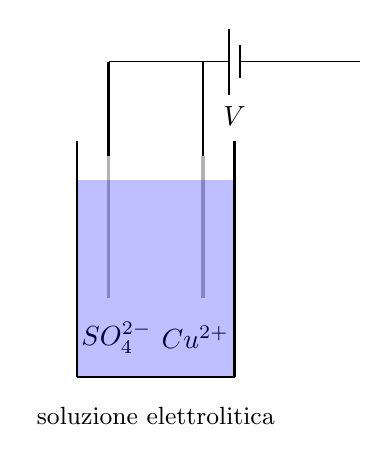
\begin{tikzpicture}[scale=1]


% --- Elettrodi ---
\draw[very thick,gray!60]
  (0.9,2.8) -- (0.9,1)
  (2.1,2.8) -- (2.1,1);

\draw[thick]
  (0.9,2.8) -- (0.9,4)
  (2.1,2.8) -- (2.1,4);

\draw (0.9,4) to[battery1,l_=$V$] (4.1,4);

% --- Etichette ---
\node at (1,0.5) {$SO_4^{2-}$};
\node at (2,0.5) {$Cu^{2+}$};
\node at (1.5,-0.5) {\small soluzione elettrolitica};

\begin{scope}[shift={(0.5,0)}]
     \fill[blue, opacity=0.25] (0,0) -- (2,0) -- (2,2.5) -- (0,2.5) -- cycle;
    \draw[thick] (0,0) -- (0,3); 
    \draw[thick] (0,0) -- (2,0); 
    \draw[thick] (2,0) -- (2,3); 
 
\end{scope}

\end{tikzpicture}
\end{center}





\end{document}
